\lecture{10. For They Shall All Know Me}{10}

%------------------------------------------------------------------------------
\section{Introduction}

%--------------------------------------
\begin{frame}
\frametitle{Do you know what this is?}
\begin{center}
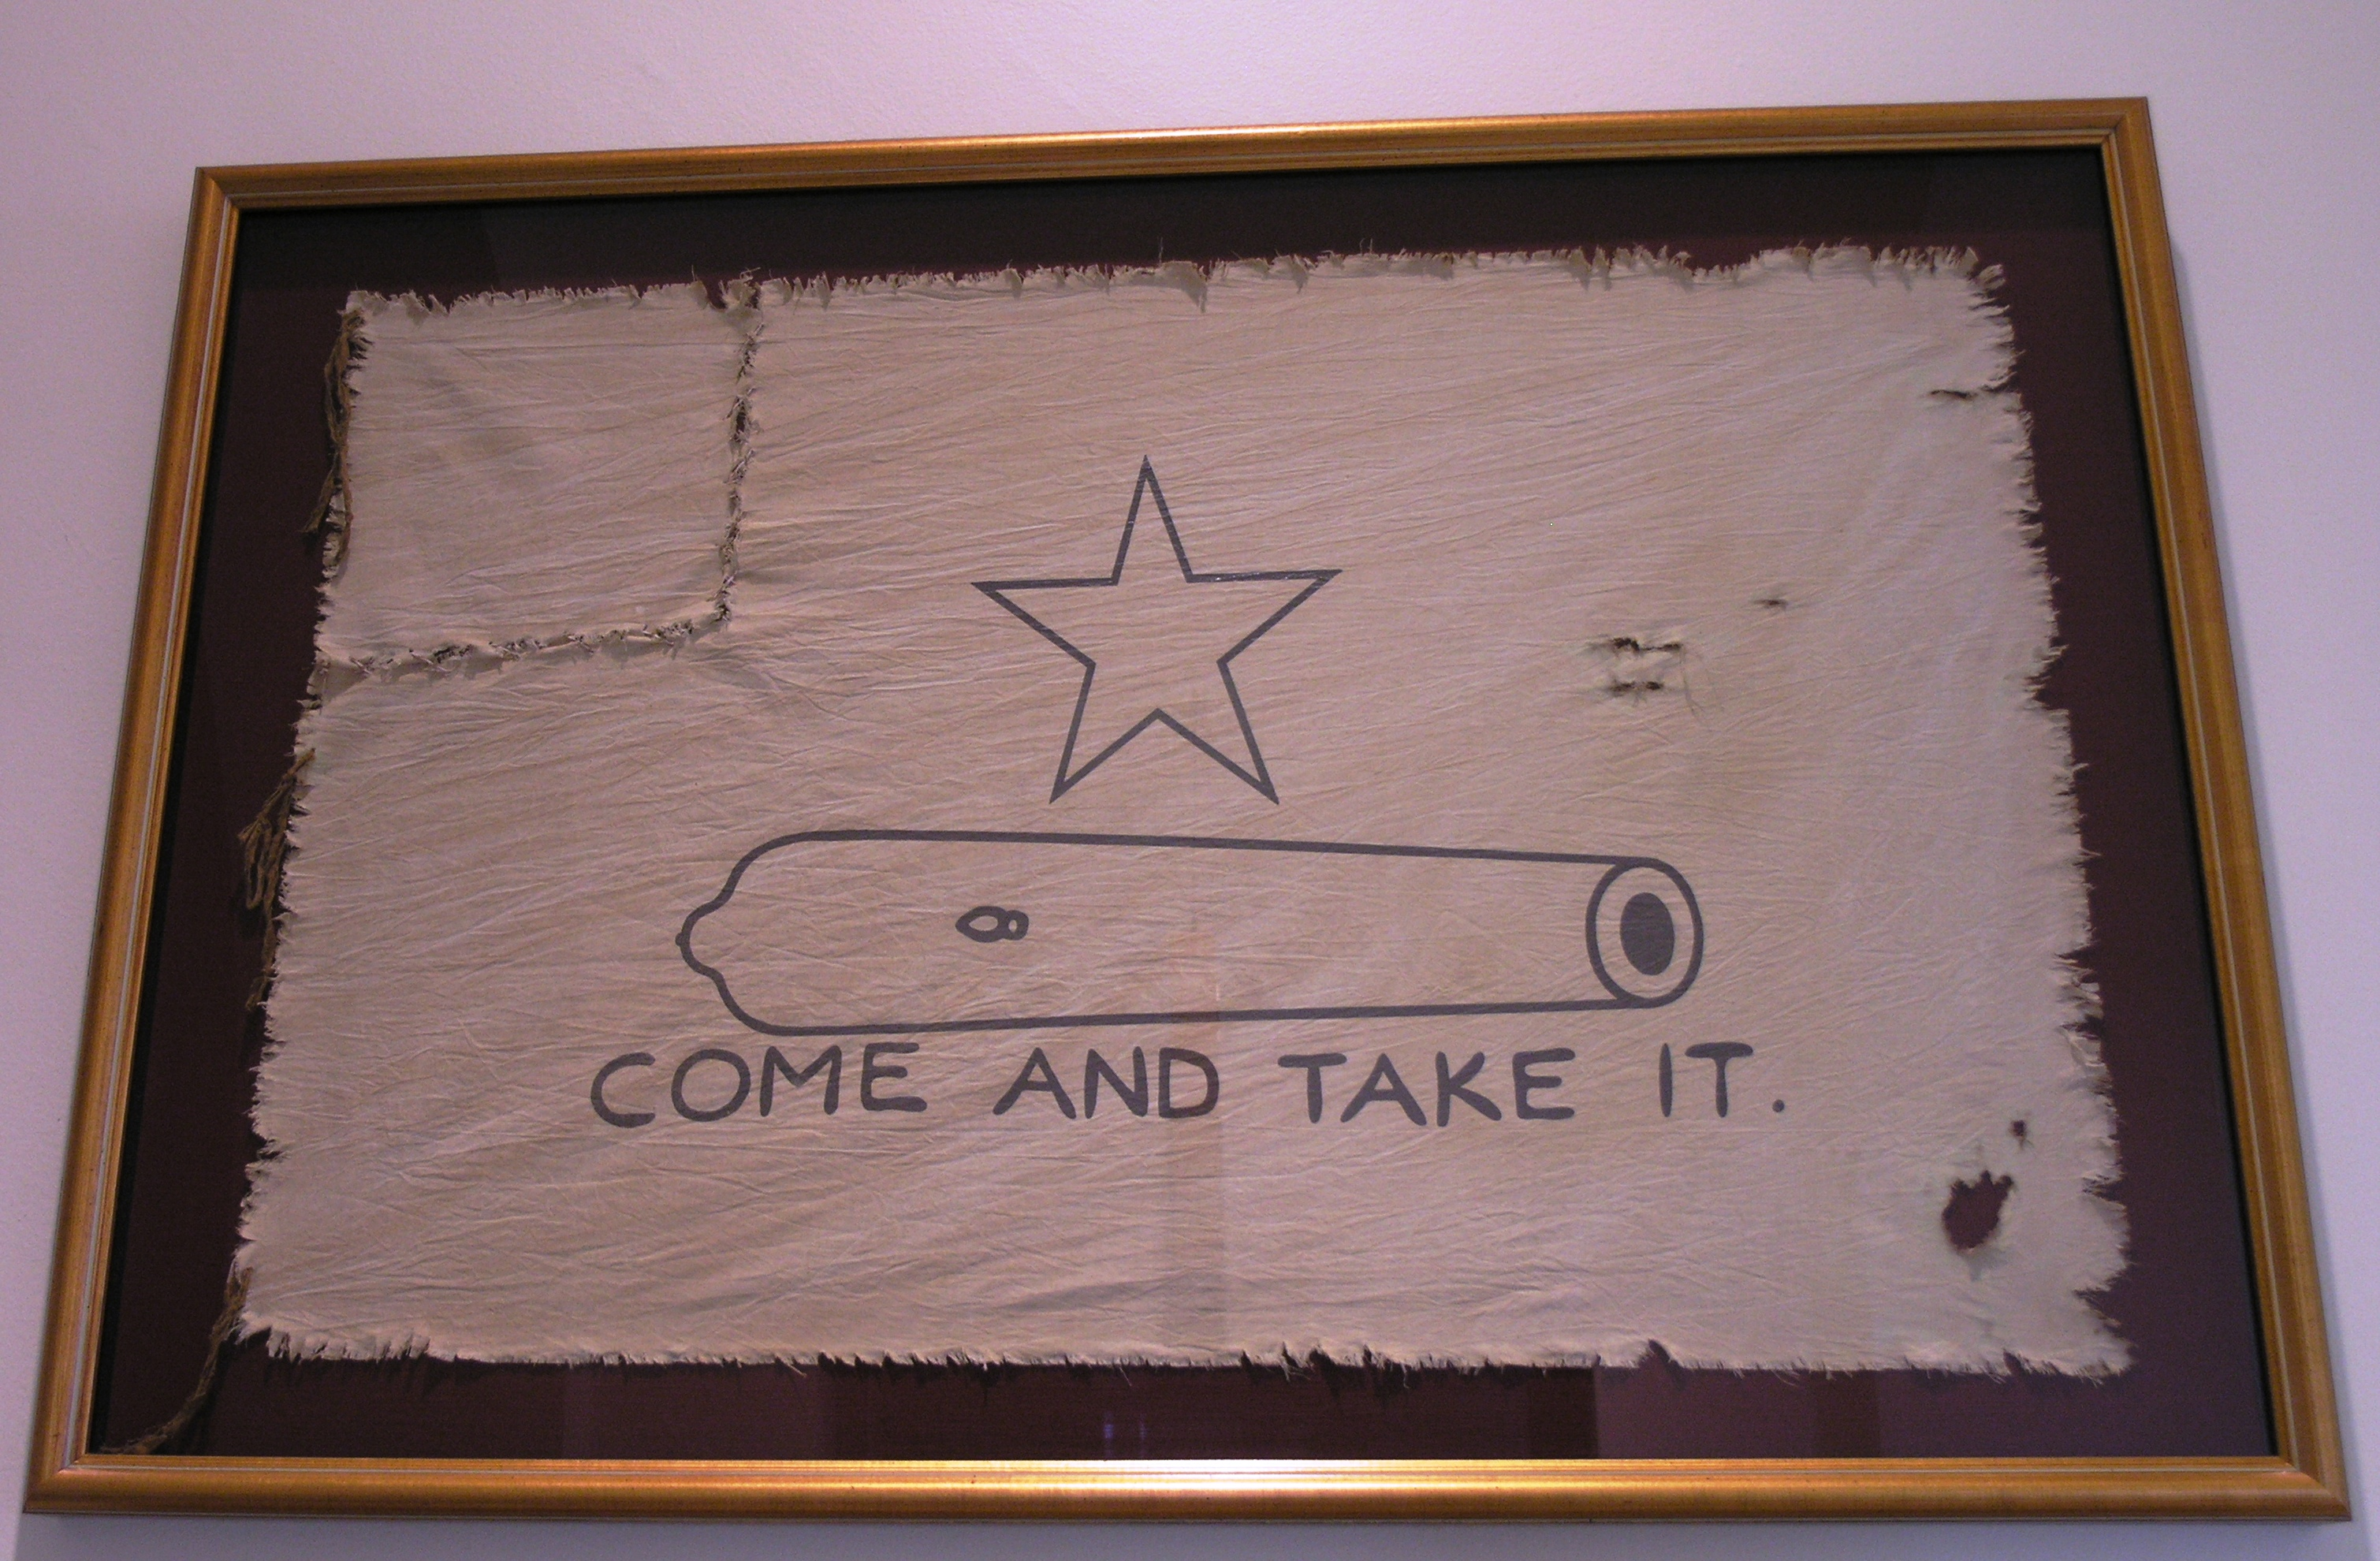
\includegraphics[width=.9\textwidth]{figures/comeAndTakeIt.jpg}
\end{center}
\note[item]{Those of you -- rightly or wrongly -- involved in the teaparty or in defending gun rights probably recognize this flag with the star and canon on it and with the motto `Come and Take It'.}
\note[item]{This flag has been co-opted by those groups to represent resistance against the over-reach of big government.}
\note[item]{But, do you `know' what this flag is and where it comes from}
\note[item]{This flag, which hangs in the Texas state capitol building, is a replica of the original flag that hung over the town of Gonzales, Texas.}
\note[item]{It marks the beginning of the Texas revolution against Mexico.}
\note[item]{The star on this flag is the same star that's present in the Texas flag.}
\note[item]{There's a difference between knowing and \emph{knowing}}.
\end{frame}


%--------------------------------------
\begin{frame}{God wants a relationship with people}
\framesubtitle{Jeremiah 31:31-34}
	\keyversehiglight{And no longer shall each one teach his neighbor and each his brother, saying, `Know the Lord,' for they shall all know me}
	
\note{09:32}
\end{frame}

%--------------------------------------
\begin{goals}
\goal Show that God's people are now joined by a common faith not a common ancestry 
\goal Elaborate on what it means to `know' God
\goal Come up with a plan to know God better

\note{09:33}
\end{goals}

%------------------------------------------------------------------------------
\section{Faith not Ancestry}

%--------------------------------------
\begin{frame}{No longer shall each one teach his neighbor}
\framesubtitle{Jer. 31:34}

\emph{`And all that generation also were gathered to their fathers. And there arose another generation after them who did not know the Lord or the work that he had done for Israel.'} Judges 2:10

\begin{itemize}
	\item The judges generation were still God's chosen people, but they didn't know God.
	\item This situation is not possible under the New Covenant
	\item You can't join God's people unless you know the gospel.
\end{itemize}

\note{09:36}
\note[item]{We had a question about this at the beginning of the class.}
\note[item]{One could misread Jer. 31:34 to say that everyone is going to get a special revelation that leads them to faith in Jesus Christ.}
\note[item]{That's not the case.}
\end{frame}

%--------------------------------------
\begin{frame}{Abraham is our father}
\framesubtitle{Rom 4:1-25}

\begin{itemize}
	\item Abraham was counted righteous before he was circumcised -- the sign shared by the Israelites. (v11)
	\item His faith was that God would fulfill his promises.
	\item Abraham is the father of those who share his faith.
\end{itemize}

\note{09:40}
\end{frame}

%--------------------------------------
\begin{frame}{Faith allows for forgiveness}
\framesubtitle{Rom 4:1-25}

\begin{itemize}
	\item When we attempt justification by works, then we receive rewards equal to our righteousness. (v.4)
	\item That puts us all in a bad place. (v.15)
	\item Faith allows God's promises to rest on grace. (v.16)
	\item Righteousness is counted to us who believe in God and His resurrection of Jesus. (v.23-25)
\end{itemize}

\note{09:44}
\note[item]{We've already talked about how faith is important}
\end{frame}

%------------------------------------------------------------------------------
\section{What is `Knowing' God?}

%--------------------------------------
\begin{frame}{Gaining Christ}
\framesubtitle{Phil. 3:3-10}

Paul's goal:
\begin{itemize}
	\item Be found \emph{in} Jesus
	\item Not having a righteousness of his own 
	\item Righteousness through faith
	\item Righteousness given by God
\end{itemize}

\note{09:48}
\note[item]{Knowing Christ is having being given righteousness from God.}
\end{frame}

%--------------------------------------
\begin{frame}{Knowing Jesus' power}
\framesubtitle{Phil. 3:3-10}

Paul's goal:
\begin{itemize}
	\item Know Jesus
	\item Know the power of his resurrection
	\item Know the fellowship of His sufferings
	\item By conforming to his death.
\end{itemize}

\note{09:52}
\note[item]{These all sound like pretty negative things}
\note[item]{What is the power of Jesus' resurrection?}
\note[item]{What is the fellowship of His suffering?}
\note[item]{How are we conformed to his death?}
\end{frame}

%--------------------------------------
\begin{frame}{Strengthened with power}
\framesubtitle{Eph. 3:14-19}

\begin{itemize}
	\item Knowing Christ requires strength (v.18)
	\item This strength comes from the Lord with power (v.16)
	\item Christ, his people, and his plan are big (v.18-19)
	\item The focal point is love (v.17-19)
\end{itemize}

\note{09:56}
\note[item]{And he will accomplish this more than we can know v. 20}
\end{frame}

%------------------------------------------------------------------------------
\section{How to know God better}

%--------------------------------------
\begin{frame}{Give up your greatness}
\framesubtitle{Phil. 3:3-10}

``I once also had confidence in the flesh\ldots, but everything that was gain to me, I have considered to be a loss because of Christ''

\note{10:00}
\end{frame}

%--------------------------------------
\begin{frame}{Pray and Listen}
\framesubtitle{Matthew 7:7-12}

\begin{itemize}
\item Keep asking, and it will be given to you. 
\item Keep searching, and you will find. 
\item Keep knocking, and the door will be opened to you. 
\item \ldots how much more will your Father in heaven give good things to those
who ask Him! 
\end{itemize}

\note{10:04}
\note[item]{Eph 3:20}
\end{frame}

%--------------------------------------
\begin{frame}{Give to others as God gives to you}
\framesubtitle{Matthew 7:7-12}

The guarantee of God's grace is followed by a command for us to show grace to others.

\note{10:08}
\note[item]{Eph. 3:17}
\end{frame}

%------------------------------------------------------------------------------
\section{Review}

\begin{frame}{For They Shall All Know Me}
	God's people share a common faith not a common ancestry 
	\begin{itemize}
		\item Israel had generations that 'knew not God'
		\item All Christians know God. 
		\item We share Abraham's faith in God and His promises.
	\end{itemize}
	`Knowing' God means\ldots
	\begin{itemize}
		\item Knowing Jesus', His resurrection, and sharing in His sufferings
		\item Being \emph{in} Jesus with a righteousness through faith
		\item Gaining strength and love to know the bigness of God's plan.
	\end{itemize}
	Know God better by\ldots
	\begin{itemize}
		\item Giving up your own greatness
		\item Prayer and study (with guaranteed success)
		\item Giving to others as God has given to you
	\end{itemize}
\note{10:12}
\end{frame}